\section{Strumentazione}
La strumentazione impiegata è quella presente sul banco di lavoro, più:
	\begin{itemize}
		\item 2 circuiti integrati SN7400 (4xNAND);
		\item il generatore di onde quadre, montato nelle precedenti esperienze;
		\item 1 DIP switch a 4 interruttori;
		\item 1 diodo 1N4148, 2 diodi led.
	\end{itemize}

\section{Circuiti logici elementari}
Si è inizialmente proceduto alla verifica della tabella di verità della porta NAND (\tab{f:NAND}), in tre modi diversi:
\begin{itemize}
	\item collegando due interruttori agli ingressi e posizionandoli nella 4 possibili combinazione (lavorando in logica TTL l'estremo di ogni interruttore va collegato a massa);
	\item collegando l’uscita o le uscite ad un diodo LED, attraverso una resistenza di limitazione di corrente;
	\item utilizzando le due uscite	sfasate di arduino, che coprono tutti gli stati possibili: la traccia dell’oscilloscopio
	in uscita rappresenta direttamente la tabella di verità.
\end{itemize}

L'integrato  SN7400 è stato alimentato con una tensione di alimentazione $V_{cc}=$\SI{ 5.01 \pm 0.03  }{\volt}.
\begin{figure}[H]
	\begin{minipage}{0.5\textwidth}
		\centering
		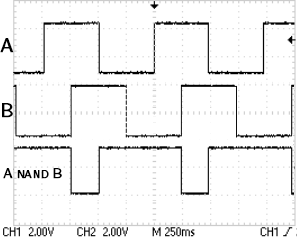
\includegraphics[scale=0.8]{../Figs-Tabs/NAND.png}
		\caption{porta NAND all'oscilloscopio}
		\label{f:NAND}
	\end{minipage}
	\begin{minipage}{0.5\textwidth}
	\centering
	\begin{tabular}{sss}
		\toprule
		A &  B & A\; NAND\; B	\\
		\midrule
		0  & 0 & 1\\
		0  & 1 & 1\\
		1  & 0 & 1\\
		1  & 1 & 0\\
		\bottomrule
	\end{tabular}
	\captionof{table}{Tabella di verità NAND.}
	\label{t:NAND}
	\end{minipage}
\end{figure}

In \fig{t:NAND} è visibile il risultato ottenuto ed è possibile verificare la tabella di verità.

\subsection{AND}
Si è montato il circuito in \figurename{ \ref{f:AND}} che presenta la tabella di verità in \tab{t:AND}.

\begin{figure}[H]
	\begin{minipage}{0.5\textwidth}
		\centering
		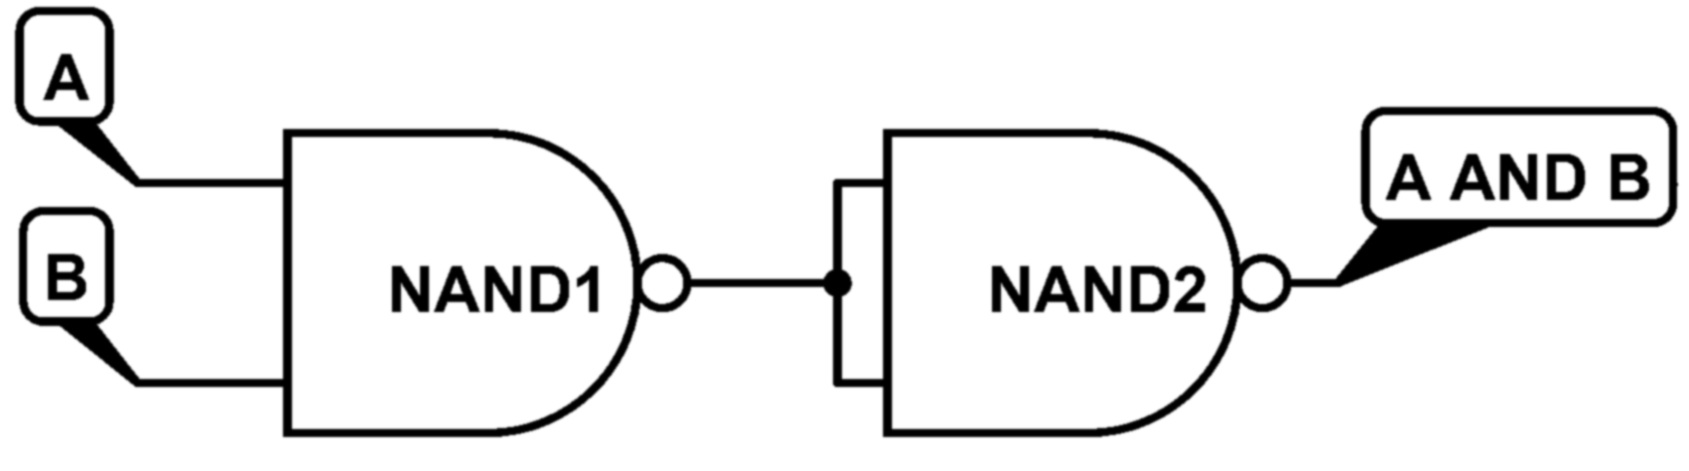
\includegraphics[scale=0.22]{../Figs-Tabs/AND_.png}
		\caption{schema porta AND}
		\label{f:AND}
	\end{minipage}
	\begin{minipage}{0.5\textwidth}
		\centering
		\begin{tabular}{ccc}
			\toprule
			A & B & A\;AND\;B	\\
			\midrule
			0  & 0 & 0\\
			0  & 1 & 0\\
			1  & 0 & 0\\
			1  & 1 & 1\\
			\bottomrule
		\end{tabular}
		\captionof{table}{Tabella di verità AND.}
		\label{t:AND}
	\end{minipage}
\end{figure}

Questa risulta a sua volta verificata dall'andamento osservato e riportato in \figurename{ \ref{f:osci-and}}

\begin{figure}[H]
	\begin{minipage}{0.5\textwidth}
		\centering
		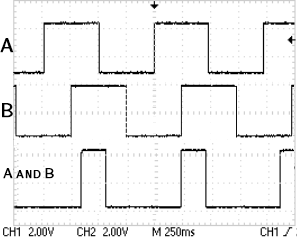
\includegraphics[scale=1]{../Figs-Tabs/and.png}
		\caption{porta AND all'oscilloscopio}
		\label{f:osci-and}
	\end{minipage}
	\begin{minipage}{0.5\textwidth}
		\centering
		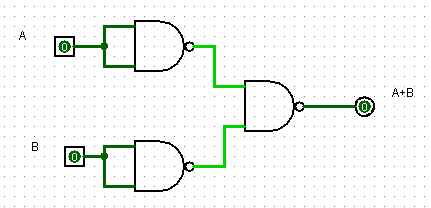
\includegraphics[scale=1]{../Figs-Tabs/or.png}
		\caption{porta OR all'oscilloscopio}
		\label{f:osci-or}
	\end{minipage}
\end{figure}

\subsection{OR}
	Per la funzione OR essendo $ OR(A,B) = A + B = \overline{\overline{(A +B)}}= \overline{(\overline{A} \cdot \overline{B})}$	è stato montato il circuito in \figurename{ \ref{f:OR}}, che presenta la tabella di verità in \tab{t:OR}.


\begin{figure}[H]
	\begin{minipage}{0.5\textwidth}
		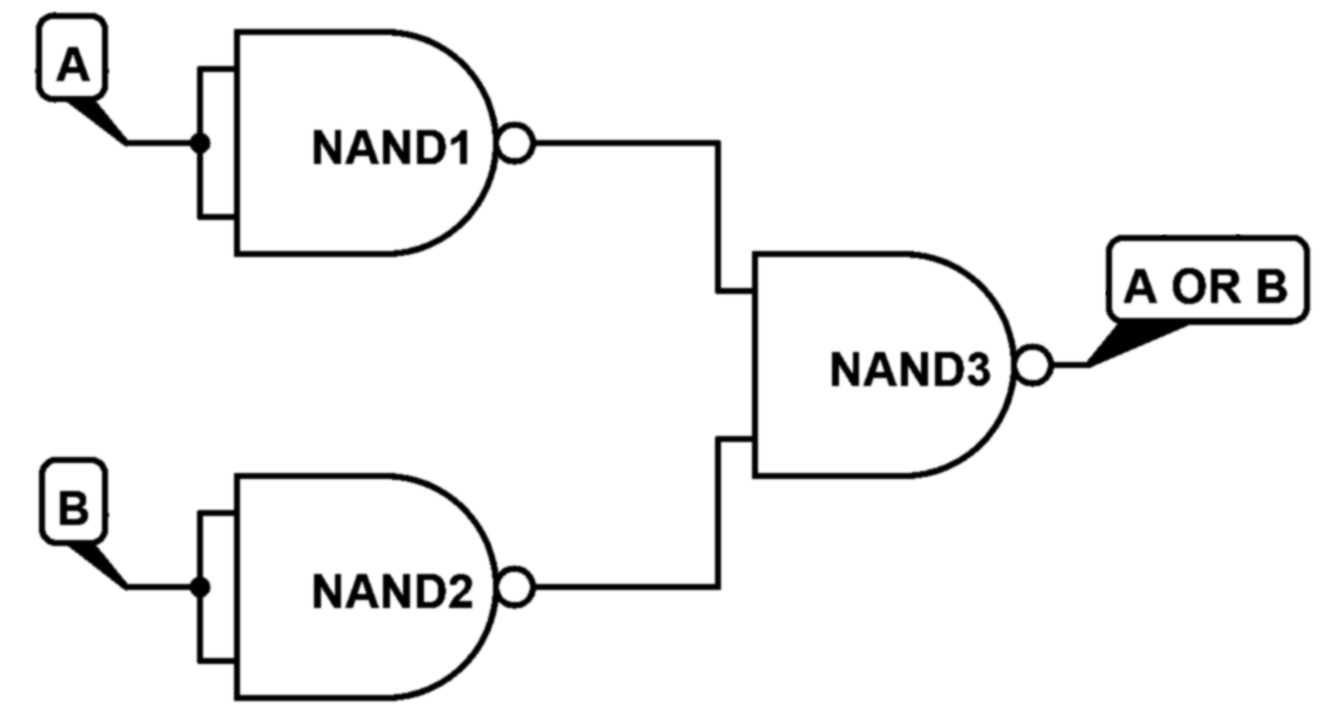
\includegraphics[scale=0.28]{../Figs-Tabs/OR_.png}
		\caption{schema porta OR}
		\label{f:OR}
	\end{minipage}
	\begin{minipage}{0.5\textwidth}
			\centering
			\begin{tabular}{sss}
				\toprule
				A & B & A\;OR\;B	\\
				\midrule
				0  & 0 & 0\\
				0  & 1 & 1\\
				1  & 0 & 1\\
				1  & 1 & 1\\
				\bottomrule
			\end{tabular}
			\caption{Tabella di verità OR.}
			\label{t:OR}
	\end{minipage}
\end{figure}

Questa risulta a sua volta verificata dall'andamento osservato e riportato in \figurename{ \ref{f:osci-or}}.
\newpage
\subsection{XOR}
	Per la funzione XOR essendo $ XOR(A,B) = A \oplus B = (A \cdot \overline{B}) + (\overline{A} \cdot B) =
	 \overline{
	 	\overline{
	 		( A \cdot \overline{
	 			(A \cdot B)
 			}	 ) \cdot
 		\overline{
 			(B \cdot \overline{
 				(A \cdot B)
 			} )
 		}
 	}
	}$,
	è stato montato il circuito in \figurename{ \ref{f:XOR}} che presenta la tabella di verità in \tablename{ \ref{t:XOR}}.

	\begin{figure}[H]
		\begin{minipage}{0.5\textwidth}
		\centering
		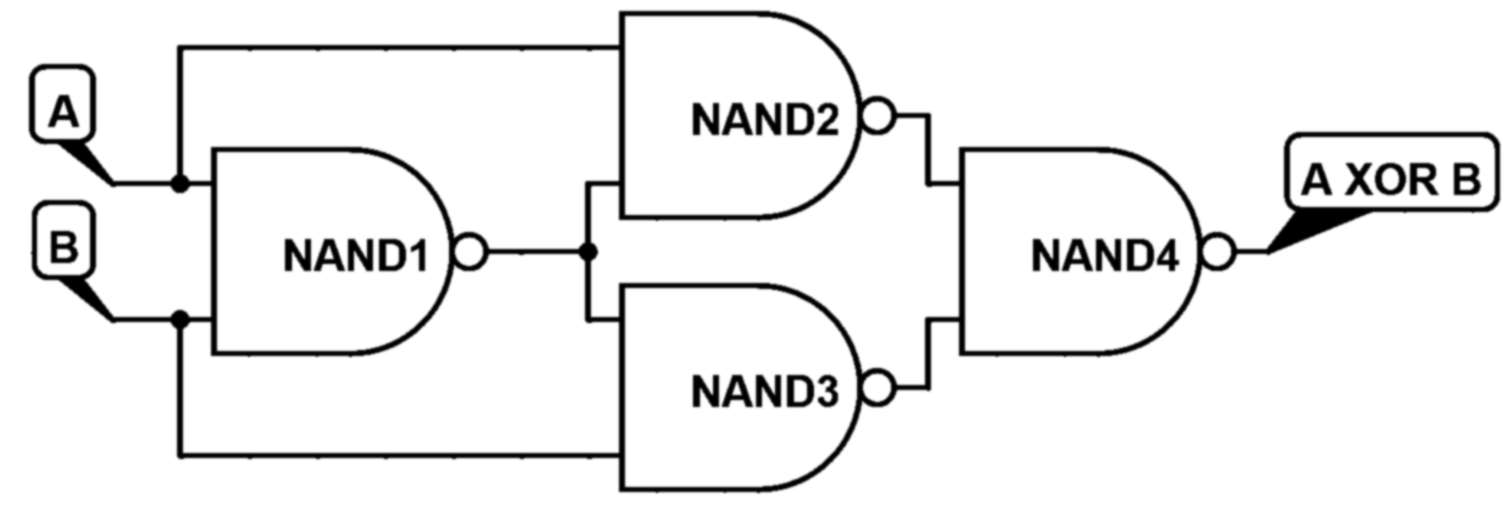
\includegraphics[scale=0.25]{../Figs-Tabs/XOR_.png}
		\caption{schema porta XOR}
			\label{f:XOR}
		\end{minipage}
		\begin{minipage}{0.5\textwidth}
		\centering
		\begin{tabular}{sss}
			\toprule
			A & B &A\; XOR\; B	\\
			\midrule
			0  & 0 & 0\\
			0  & 1 & 1\\
			1  & 0 & 1\\
			1  & 1 & 0\\
			\bottomrule
		\end{tabular}
		\caption{Tabella di verità XOR.}
		\label{t:XOR}
		\end{minipage}
	\end{figure}

Questa risulta a sua volta verificata dall'andamento osservato e riportato in \figurename{ \ref{f:osci-xor}}.

	\begin{figure}[hb]
		\centering
		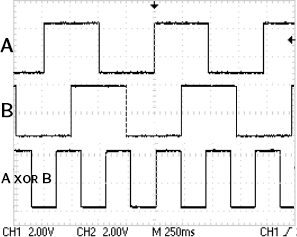
\includegraphics[scale=1]{../Figs-Tabs/xor.png}
		\caption{porta XOR all'oscilloscopio}
		\label{f:osci-xor}
	\end{figure}

\subsection{Sommatore ad un bit}
Il circuito sommatore è costituito su un uscita da una porta XOR (bit meno significativo) ed da una porta AND sull'altra uscita (bit più significativo). Si è montato pertanto il circuito in \figurename{ \ref{f:somma}} e se ne è verificato il funzionamento.
\begin{figure}[H]
	\centering
	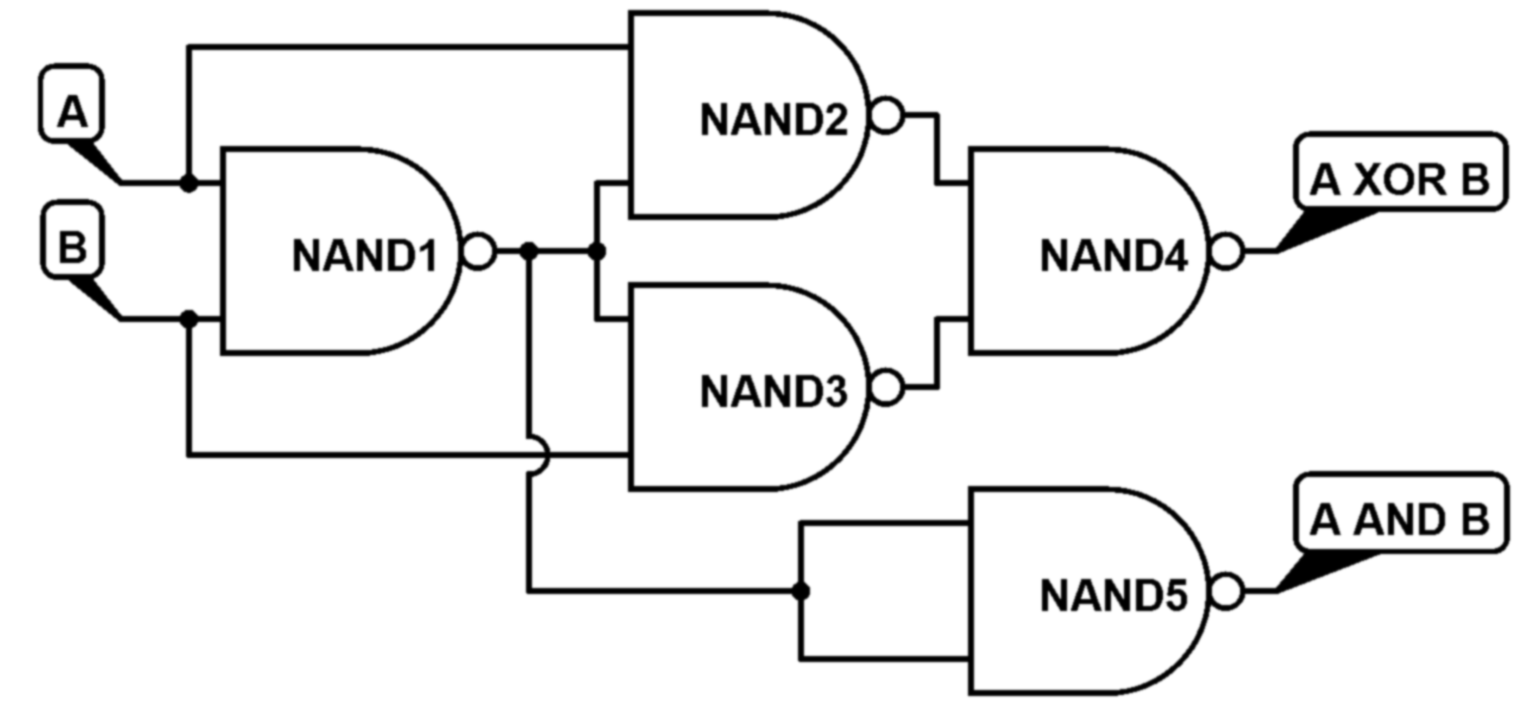
\includegraphics[scale=0.3]{../Figs-Tabs/SUM_.png}
	\caption{schema del sommatore a 1 bit}
\end{figure}\label{f:somma}
